% id: 96-15
% book: 100발100중 3-2 중간 · 01 3-2 중간(삼각비·삼각비의 활용·원과 직선·원주각·부록)
% section: 실전 모의고사 1회
% figure: crop:fig-96-15.png
% answer: ①
% answer_source: 답지(빠른정답)
% variant_level: 0 (원본 전사)
% 이 파일은 build.mjs 가 items.json 에서 만든다. 고칠 때는 items.json 을 고친다.
\smash{\raisebox{1.5mm}{\dmkichul{100발100중 3-2 중간 96쪽 15번}}}
\noindent\begin{minipage}[t]{0.58\linewidth}\vspace{0pt}\raggedright 그림과 같이 $\triangle\pt{ABC}$가 원~$\pt{O}$에 외접하고 세 점~$\pt{P}$, $\pt{Q}$, $\pt{R}$는 그 접점일 때, $x$의 값은? \mbox{[4점]}\end{minipage}\hfill\begin{minipage}[t]{0.4\linewidth}\vspace{0pt}\centering 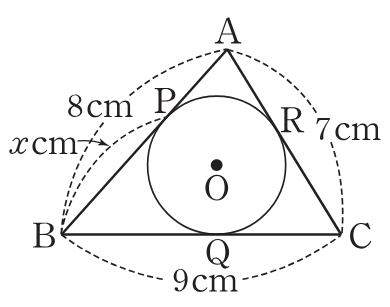
\includegraphics[width=93.5pt]{figures/fig-96-15.png}\end{minipage}\par
\begin{choicesii}{$5$}{$6$}{$7$}{$8$}{$9$}\end{choicesii}
